\let\negmedspace\undefined
\let\negthickspace\undefined
\documentclass[journal]{article}
\usepackage[a5paper, margin=10mm, onecolumn]{geometry}
\usepackage{lmodern} % Ensure lmodern is loaded for pdflatex

\setlength{\headheight}{1cm} % Set the height of the header box
\setlength{\headsep}{0mm}     % Set the distance between the header box and the top of the text

\usepackage{gvv-book}
\usepackage{gvv}
\usepackage{cite}
\usepackage{textcomp}
\usepackage{amsmath,amssymb,amsfonts,amsthm}
\usepackage{algorithmic}
\usepackage{graphicx}
\graphicspath{{./figs/}}
\usepackage{textcomp}
\usepackage{xcolor}
\usepackage{txfonts}
\usepackage{listings}
\usepackage{enumitem}
\usepackage{mathtools}
\usepackage{gensymb}
\usepackage{comment}
\usepackage[breaklinks=true]{hyperref}
\usepackage{tkz-euclide} 
\usepackage{listings}
\usepackage{gvv}                                        
\def\inputGnumericTable{}                                 
\usepackage[latin1]{inputenc}                                
\usepackage{color}                                            
\usepackage{array}                                            
\usepackage{longtable}                                       
\usepackage{calc}                                             
\usepackage{multirow}                                         
\usepackage{hhline}                                           
\usepackage{ifthen}                                           
\usepackage{lscape}
\usepackage{circuitikz}
\tikzstyle{block} = [rectangle, draw, fill=blue!20, 
text width=4em, text centered, rounded corners, minimum height=3em]
\tikzstyle{sum} = [draw, fill=blue!10, circle, minimum size=1cm, node distance=1.5cm]
\tikzstyle{input} = [coordinate]
\tikzstyle{output} = [coordinate]


\begin{document}
	
	\bibliographystyle{IEEEtran}
	\vspace{3cm}
	
\title{1.10.2}
\author{EE25BTECH11047 - RAVULA SHASHANK REDDY}
\maketitle
\hrulefill
\bigskip 

\renewcommand{\thetable}{\theenumi}
\setlength{\intextsep}{10pt}
\textbf{Question:} \\ 

  Find the unit vector in the direction of the sum of the vectors
$\vec{a} = 2\hat{i} - \hat{j} + \hat{k}$, 
$\vec{b} = 2\hat{j} + \hat{k}$.\\


\textbf{Solution:}\\

Given
\begin{align}
\vec{a} = \myvec{ 2 \\ -1 \\ 1 }\\ 
\vec{b} = \myvec{ 0 \\ 2 \\ 1 }.
\end{align}

Sum of the vectors:
\begin{align}
\vec{a}+\vec{b} = \myvec{ 2 \\ -1 \\ 1 } + \myvec{ 0 \\ 2 \\ 1 }
= \myvec{ 2 \\ 1 \\ 2 }.
\end{align}

Norm of $\vec{a}+\vec{b}$ :
\begin{align}
\|\vec{a}+\vec{b}\| = \sqrt{ \myvec{ 2 & 1 & 2 } 
\myvec{ 2 \\ 1 \\ 2 } }
= \sqrt{ 2\cdot 2 + 1\cdot 1 + 2\cdot 2 }
= \sqrt{9} = 3.
\end{align}

Using the unit vector formula :
\begin{align}
\vec{u} = \frac{\vec{a}+\vec{b}}{\|\vec{a}+\vec{b}\|}\\
\vec{u}= \frac{1}{3} \myvec{ 2 \\ 1 \\ 2 }.
\end{align}
\begin{align}
\therefore
\vec{u} = \myvec{\frac{2}{3} \\  \frac{1}{3} \\ \frac{2}{3} }
\end{align}
\newpage
\begin{figure}
    \centering
    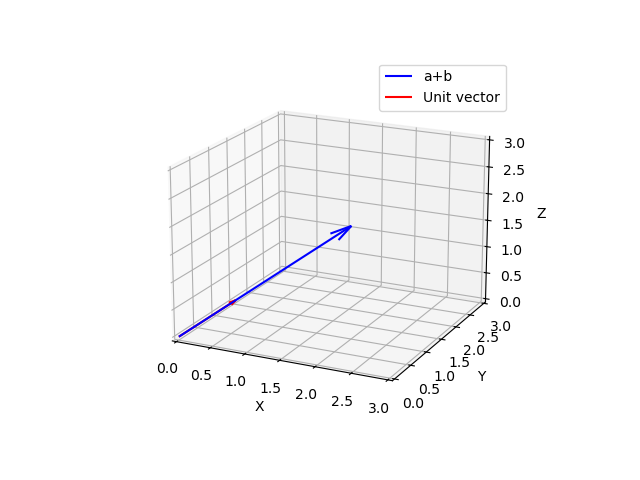
\includegraphics[width=1.0\linewidth]{fig-1.png}
    \caption{}
    \label{fig:placeholder}
\end{figure}

\end{document}